\documentclass[10pt,letter]{article}
\usepackage[utf8]{inputenc}
\usepackage{amsmath}
\usepackage{amsfonts}
\usepackage{amssymb}
\usepackage{graphicx}
\usepackage[margin=1in]{geometry}
\usepackage{float}


\begin{document}

\begin{titlepage}
\title{PHYS 5794 Homework 9}
\date{April 20, 2016}
\author{Thomas Edwards}
\maketitle
\end{titlepage}

\section{Problem 1}

\subsection{Problem Statement}
Write a Monte Carlo simulation program for the Ising model on the square lattice $L \times L$, in order to
obtain the average magnetization per site $\left< |m| \right>$ (not $\left<m\right>$), magnetic susceptibility $\chi$ as a function of
temperature $(T =1.7, 2.0, 2.14, 2.2, 2.35, 2.45, 2.75,$ and $3.3)$ for two different lattice sizes such as
$L =5$ and $12$. Notice that in the simulation we set $J = 1$ and $k_B = 1$. Use the Metropolis transition
rate. Use the periodic boundary conditions for the vertical and horizontal directions. One Monte
Carlo step (MCS) is a single-spin flip attempt, where one Monte Carlo step per spin (MCSS) is $L^2$
times one MCS. It will be easier to work with MCSS for the program. Outermost loop considers
Monte Carlo sweeps with an MCSS index, while inner loops take care of the sweeping the square
lattice sites.

$$ \left< |m| \right> = \frac{1}{M} \sum_{i=1}^M\left| \frac{1}{L^2} \sum_{j=1}^{L^2}S_j^{(i)}\right|, $$
$$\left< m^2 \right> = \frac{1}{M} \sum_{i=1}^M\left( \frac{1}{L^2} \sum_{j=1}^{L^2}S_j^{(i)}\right)^2, $$
$$\chi = \frac{\left< m^2 \right> L^2}{k_BT},T > T_c $$
$$\chi = \frac{\left< m^2 \right>-\left< |m| \right>^2}{k_BT} L^2,T < T_c $$

where $T_c = 2.269J/k_B$ and $M$ is the total MCSS. Here the sum over $i$ means that you must skip first
about 500-1000 MCSS ($n_1 =$500-1000 MCSS) and collect the data with an interval $n_0$ (in units of
MCSS). A good value of M in the sum is about 30000-100000 MCSSs. It is a good idea to start with
a small M value first and increase the M value to see if the thermal average does not significantly
change.

Plot the average magnetization per site $\left< |m| \right>$ and susceptibility $\chi$ as a function of temperature for
the two different lattice sizes. You need to plot two figures. One figure is for the magnetization and
the other figure is for the susceptibility. Compute the standard deviation of $\left< |m| \right>$.

Plot the cumulant $U_L$ as a function of temperature for three lattice sizes $L = 5, 9, $ and 12. Estimate
the critical temperature from a plot of $U_{L_1}$/$U_{L_2}$ vs temperature. The definition of the cumulant is
in the lecture notes. $U_{L_1}$/$U_{L_2}$
is a ratio of two cumulant values at different lattice sizes $L_1$ and $L_2$.
Is your $T_c$ close to the known value, 2.269?


\subsection{Method}

This problem was solved using the Monte Carlo method. In essence, the method works as follows:

\begin{itemize}
\item Initialize a lattice of $L^2$ spins with some configuration. In this example, the spins in the lattice were all initialized in the spin-down configuration (-1).
\item In a typewriter fashion, go to each spin and compute the change in energy $\Delta E$ caused by flipping that spin using the nearest neighbors in each direction ($x$ and $y$). In this problem, periodic boundary conditions were used.
\item Select a random point $\zeta$ in the domain $x \in [0,1)$.
\item If $\zeta$ is less than $W(\Delta E)$, flip the spin at the current location. $W(\Delta E)$ in this case is the Metropolis transition function, defined as
$$e^{-\Delta E/T}, \Delta E>0$$
$$1, \Delta E<=0$$
\item Continue this problem for each point in the lattice. Each full lattice run is considered one MCS run.
\item This process continues for a given number of MCS runs (chosen in this case to be 5000 non-skipped runs), skipping those that would cause autocorrelation.
\end{itemize}

One you have your set of configurations, select a subset of them such that the configurations are not correlated. In this problem, we skipped the first 10 configurations, and began with $m_10$, and then continued by skipping every 10 configurations (for example, $m_{20}, m_{30},$ etc. )

Further, we also calculate the standard deviation of the sample mean by finding 

$$ \sigma = \sqrt{ \frac{\left\langle m^2 \right\rangle - \left\langle |m| \right\rangle^2}{M}},$$


In order to determine the number of points to skip, the autocorrelation function is determined and plotted separately. This is done by finding

$$C(l) = \frac{\left\langle m_{t+l}m_{t} \right\rangle - \left\langle m_{t}\right\rangle^2  }{\left\langle m^2_{t}\right\rangle - \left\langle m_{t}\right\rangle^2} $$

$C(l)$ was solved for a number of values of $l$ (not to be confused with $L$), and the results of a sample run are shown below.

\begin{figure}[H]
  \centering
    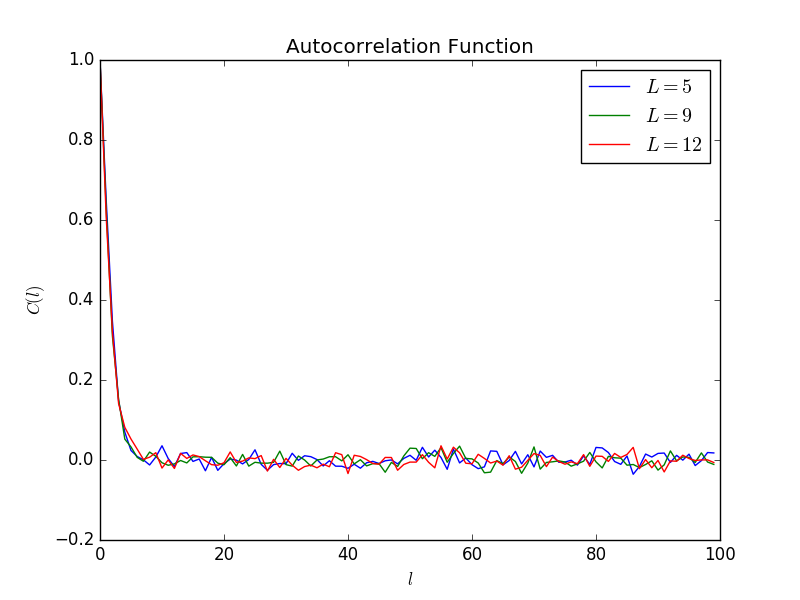
\includegraphics[width=.6\textwidth]{homework9_problem2_plot0}
\end{figure}

From here, we decide that $l=15$, just to give a significant amount of time for the values to anticorrelate. In addition, it was decided that the first 100 MCSS were skipped, just to make sure.

In addition, the cumulant for each lattice size $L$ was calculated, given by
$$ U_L = 1-\frac{\left< m^4 \right>}{3\left< m^2 \right>^2}$$

\subsection{Verification of Program}

This program was verified by comparing it to the known critical c=temperature $T_c$, which is $2.269$. In addition, the other parameters were compared to the plots from the lecture notes and discussed with the instructor to confirm that they were correct.

\subsection{Data}

The data from this program is in the plots below.
\begin{figure}[H]
  \centering
    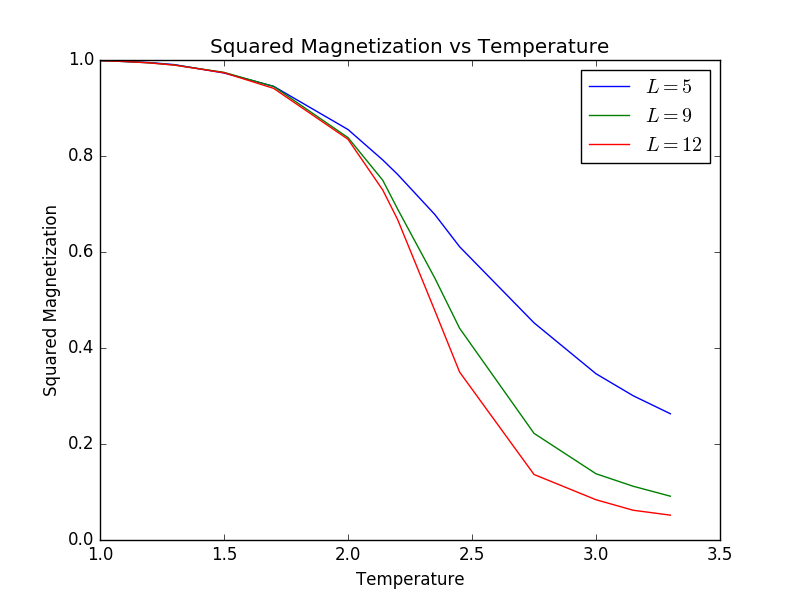
\includegraphics[width=.6\textwidth]{homework9_problem1_plot1}
\end{figure}
\begin{figure}[H]
  \centering
    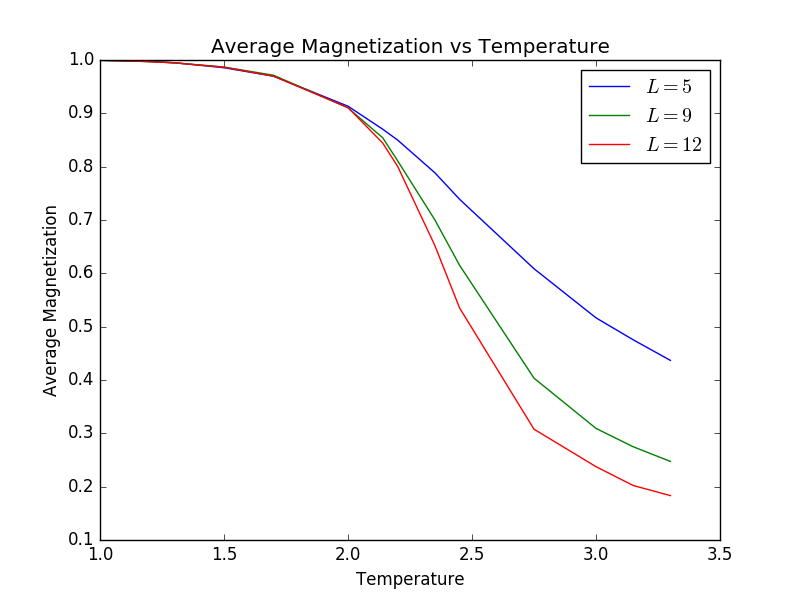
\includegraphics[width=.6\textwidth]{homework9_problem1_plot2}
\end{figure}
\begin{figure}[H]
  \centering
    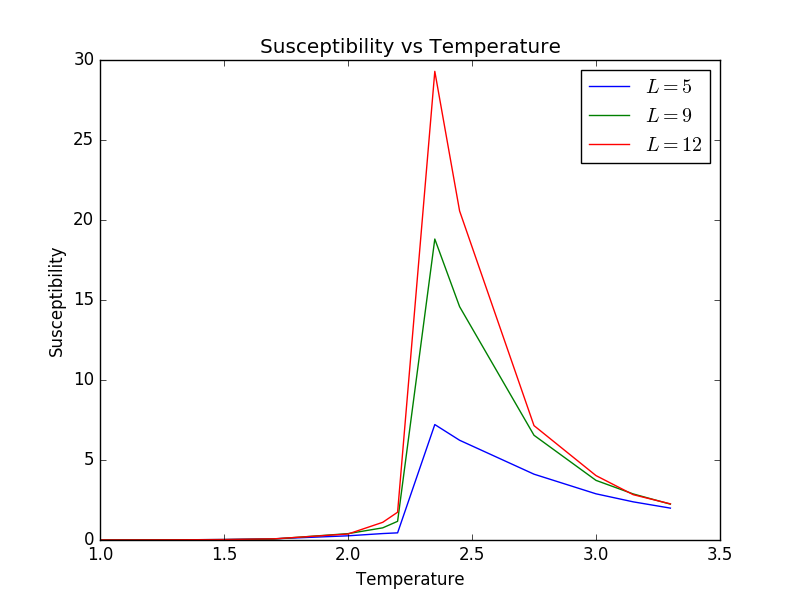
\includegraphics[width=.6\textwidth]{homework9_problem1_plot3}
\end{figure}
\begin{figure}[H]
  \centering
    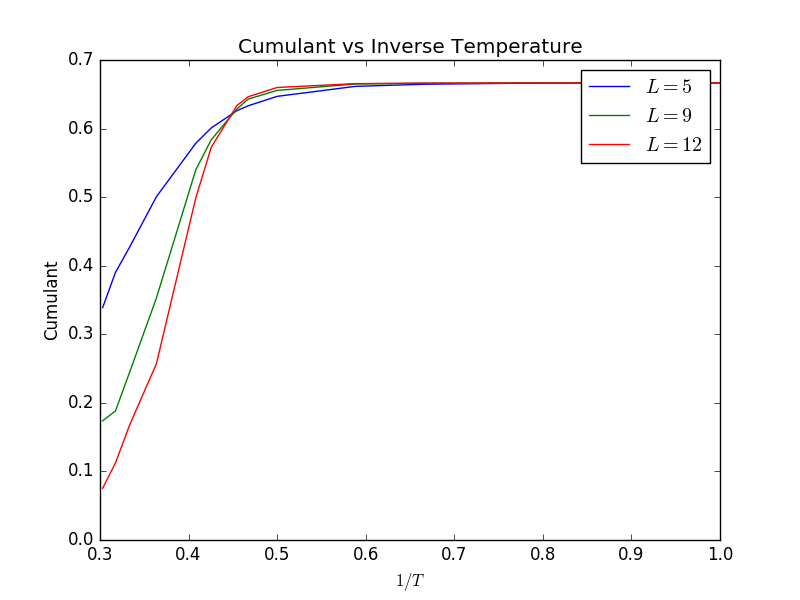
\includegraphics[width=.6\textwidth]{homework9_problem1_plot4}
\end{figure}
\begin{figure}[H]
  \centering
    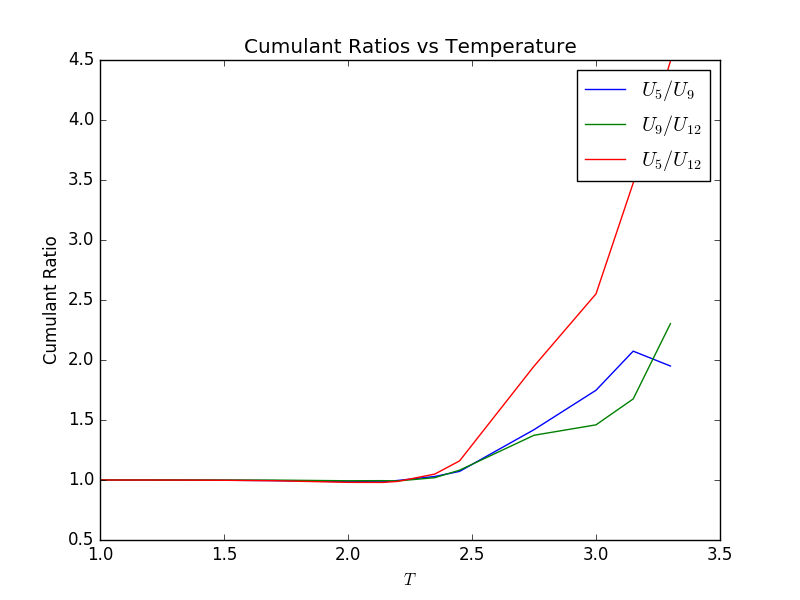
\includegraphics[width=.6\textwidth]{homework9_problem1_plot5}
\end{figure}
\begin{figure}[H]
  \centering
    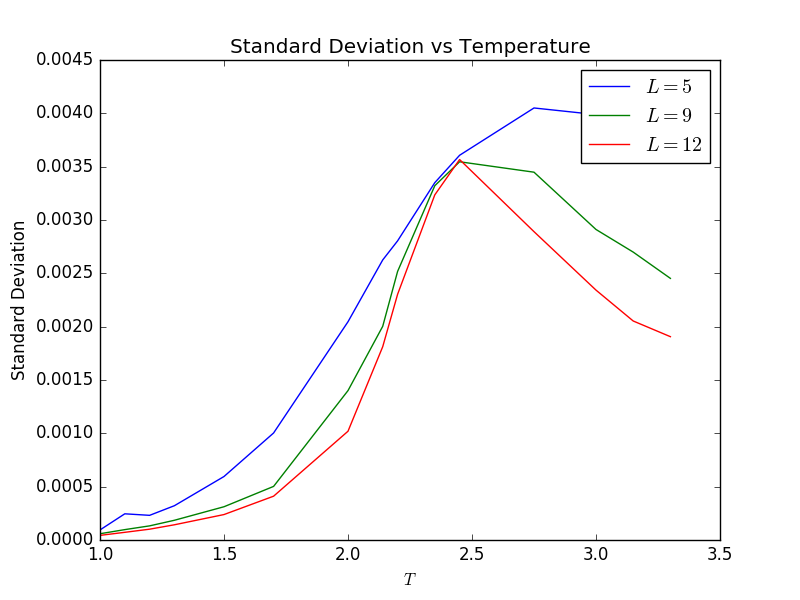
\includegraphics[width=.6\textwidth]{homework9_problem1_plot6}
\end{figure}
\subsection{Analysis and Interpretation}

From the data above, we see that the Monte Carlo method is a reasonable for solving this problem. Both the average and squared magnetization changes from a purely ordered state at low temperatures to a disordered state past the critical temperature. Further, the susceptibility appears to become discontinuous at the critical temperature, shown by the increasing magnitude of the peak as the lattice size is increased. The cumulants also appear to be as expected, leveling off at $2/3$ for low temperatures and splitting for high temperature systems.

Plotting the cumulant ratios also gives reasonable results, as they appear to diverge at approximately 2.25, which is very close to what the known value is. Finally, the standard deviation has an apparent increase as the temperature gets larger, but has a sudden and large turn after the critical temperature.

\subsection{Log}

This problem took approximately 15 hours.

\end{document}